\documentclass{sig-alternate-05-2015}
\usepackage[obey]{fixacm}

%\usepackage[margin=1in]{geometry}
%\usepackage{listings}
\usepackage[english]{babel}
%\usepackage{graphicx}
\usepackage{caption}
\usepackage{accents}
\usepackage[list=true,listformat=simple]{subcaption}
\usepackage{color,colortbl}
\definecolor{almond}{rgb}{0.94, 0.87, 0.8}
\usepackage{hyperref}

% For maintaining extended abstract and full versions of a paper.
% Usage: \ifabstract short text [\else long  text] \fi
%        \iffull     long  text [\else short text] \fi
% Uncomment the line ``\abstractfalse'' to enable the full version.
\newif\ifabstract
%\abstracttrue
\abstractfalse
\newif\iffull
\ifabstract \fullfalse \else \fulltrue \fi

\ifabstract  %squish
\usepackage{times}

% Compact mainlevel section titles, using \paragraph's while keeping numbering,
% but without \appendix support.
%{\makeatletter
% \gdef\section{\@ifnextchar*\section@star\section@normal}
% \gdef\section@normal#1{\refstepcounter{section}%
%   \paragraph{\arabic{section}\hbox{~~}#1.}%
%   \addcontentsline{toc}{section}{\protect\numberline{\arabic{section}}{#1}}}
% \gdef\section@star*#1{\paragraph{#1.}}}

% Compact subsection titles, using \paragraph's while keeping numbering.
%{\makeatletter
% \gdef\subsection{\@ifnextchar*\subsection@star\subsection@normal}
% \gdef\subsection@normal#1{\refstepcounter{subsection}%
%   \paragraph{\thesubsection\hbox{~~}#1.}%
%   \addcontentsline{toc}{subsection}{\protect\numberline{\thesubsection}{#1}}}
% \gdef\subsection@star*#1{\paragraph{#1.}}}

% Redefine paragraph to have no leading space, but rather indent.
%{\makeatletter
% \gdef\paragraph{\@startsection{paragraph}{4}{\parindent}{-0pt}{-1em}
%   {\normalfont\normalsize\bfseries}}}

% Tighter version of just \paragraph.
%\newlength\aboveparagraphskip
%\aboveparagraphskip=3.25ex plus 1ex minus .2ex
%\newlength\belowparagraphskip
%\belowparagraphskip=-1em
%\makeatletter
%\def\paragraph{\@startsection{paragraph}{4}{\z@}{-\aboveparagraphskip}%
%                 {\belowparagraphskip}{\normalfont\normalsize\bfseries}}
%\makeatother
%\aboveparagraphskip=.5ex plus .5ex minus .25ex

% Remove periods at ends of paragraphs in ACM sig-alternate format.
{\makeatletter\gdef\@period{}}

% Simple \paragraph in particular to clean up ACM sig-alternate format.
\def\paragraph#1{\par\textbf{#1} }

\fi

\usepackage[
	counters = {theorem},
	%title = {Omitted\ Proofs},
	abstract, appendix
]{magicappendix}

% Force \boldmath in \section etc. titles without upsetting hyperref.
% Warning: Redefines all instances of \bfseries to turn on \boldmath too.
\let\realbfseries=\bfseries
\def\bfseries{\realbfseries\boldmath}

\urlstyle{same}

\newtheorem{theorem}{Theorem}[section]
\newtheorem{lemma}[theorem]{Lemma}
\newtheorem{proposition}[theorem]{Proposition}
\newtheorem{corollary}[theorem]{Corollary}

\newcommand{\ul}[1] {\underline{#1}}

\newenvironment{definition}[1][Definition]{\begin{trivlist}
\item[\hskip \labelsep {\bfseries #1}]}{\end{trivlist}}
\newenvironment{example}[1][Example]{\begin{trivlist}
\item[\hskip \labelsep {\bfseries #1}]}{\end{trivlist}}
\newenvironment{remark}[1][Remark]{\begin{trivlist}
\item[\hskip \labelsep {\bfseries #1}]}{\end{trivlist}}

% Complex \xxx for making notes of things to do.  Use \xxx{...} for general
% notes, and \xxx[who]{...} if you want to blame someone in particular.
% Puts text in brackets and in bold font, and normally adds a marginpar
% with the text ``xxx'' so that it is easy to find.  On the other hand, if
% the comment is in a minipage, figure, or caption, the xxx goes in the text,
% because marginpars are not possible in these situations.
{\makeatletter
 \gdef\xxxmark{%
   \expandafter\ifx\csname @mpargs\endcsname\relax % in minipage?
     \expandafter\ifx\csname @captype\endcsname\relax % in figure/caption?
       \marginpar{xxx}% not in a caption or minipage, can use marginpar
     \else
       xxx % notice trailing space
     \fi
   \else
     xxx % notice trailing space
   \fi}
 \gdef\xxx{\@ifnextchar[\xxx@lab\xxx@nolab}
 \long\gdef\xxx@lab[#1]#2{\textbf{[\xxxmark #2 ---{\sc #1}]}}
 \long\gdef\xxx@nolab#1{\textbf{[\xxxmark #1]}}
 % This turns them off:
 %\long\gdef\xxx@lab[#1]#2{}\long\gdef\xxx@nolab#1{}%
}


% Compact list environments.  Note that itemize* and enumerate* use the
% same counters and symbols as the usual itemize and enumerate environments.
%\def\compactify{\itemsep=0pt \topsep=0pt \partopsep=0pt \parsep=0pt}
\let\latexusecounter=\usecounter
\newenvironment{itemize*}
  {\begin{itemize}\compactify}
  {\end{itemize}}
\newenvironment{enumerate*}
  {\def\usecounter{\compactify\latexusecounter}
   \begin{enumerate}}
  {\end{enumerate}\let\usecounter=\latexusecounter}
\newenvironment{description*}
  {\begin{description}\compactify}
  {\end{description}}

% Put figures and text together
\def\textfraction{0.01}
\def\topfraction{0.99}
\def\dbltopfraction{0.99}
\def\bottomfraction{0.99}
\def\floatpagefraction{0.99}
\def\dblfloatpagefraction{0.99}
\def\dbltopnumber{100}

% Fonts
\def\id#1{\textit{#1}}
\def\proc#1{\textsc{#1}}
\let\epsilon=\varepsilon
\let\keyw=\textbf


\begin{document}

\title{Discriminating Sound Textures}


\numberofauthors{2} 

\auskip=0.5\auskip

\author{
\alignauthor
  Jayson Lynch \\
  \affaddr{MIT CSAIL}\\
       \affaddr{32 Vassar Street}\\
       \affaddr{Cambridge, MA 02139}\\
       \email{jaysonl@mit.edu}
\alignauthor Eric Mannes\\
\affaddr{MIT CSAIL}\\
       \affaddr{32 Vassar Street}\\
       \affaddr{Cambridge, MA 02139}\\
       \email{mannes@mit.edu}
       }

\maketitle
\begin{abstract}
In this paper we investigate a feature set for the classification of sound textures based on signal compressibility, sparsity, and temporal homogeneity. The feature set was examined and used in a classifier for sound textures. We show that for sound samples with normalized amplitude, these features have very little predictive power with respect to whether a sound is textural. 
\end{abstract}

\keywords{Machine Learning, Sound Textures, Human Audition}

\section{Introduction} 
This paper explores a new feature set for audio classification. Specifically, we look at a feature ensemble related to compressibility, sparsity, and temporal homogeneity in the problem of classifying audio signals as \emph{sound textures}. Sound textures, such as rain or crackling fire, are the result of many similar acoustic events. These sounds seem to form a cohesive auditory category which might be processed by the brain in a distinct fashion\cite{mcdermott2013summary, McDermott2011926}. Their study has partially been motivated by the analogous visual textures which comprise a significant body of literature. Tomita and Tsuji provide a book on the computational analysis of visual textures\cite{tomita2013computer}. The ideas that visual textures may be characterized by simple statistical features\cite{julesz1962visual} or atomistic units\cite{julesz1981textons} is carried over into some of the theory of sound textures. Recent work by McDermott and Simoncelli show many sound textures are well characterized by their time-averaged statistical properties\cite{McDermott2011926, mcdermott2013summary}. Saint-Arnaud's Master's Thesis attempts to extract the sound atoms that make up sound textures and use this as a basis for a classifier\cite{saint1995classification}. The thesis also discusses human perception of sound textures and the difficulties surrounding a good definition. A significant amount of the machine learning work in sound textures has been around synthesis often using wavelet hierarchies\cite{kersten2010sound} or sound atoms\cite{saint1995analysis}. Schwarz provides a general overview of methods as well as a classification scheme of the synthesis methods used\cite{schwarz2011state}.

McDermott and Simoncelli work shows that for many sound textures, the salient features that cause humans to classify these sounds are controlled by a number of time-averaged statistics of the sounds\cite{McDermott2011926, mcdermott2013summary}. This leads to an interesting question of why some sounds seem to be identified by time-averaged properties, when many other, such as speech or music, depend strongly on their temporal structure. McDermott et. al. conjecture that the `sparsity' or `compressibility' are related to the sounds that are perceived in this way. In addition, they mention that sound textures are `temporally homogeneous' without giving formal definitions of these terms. This paper seeks to build upon these ideas both to investigate new features for audio classification as well as to lend evidence toward the previous conjectures about sound texture perception. We provide several formal definitions of audio compressibility, sparsity, and temporal homogeneity in Section~\ref{sec:definitions}. These are then extracted as a feature set and are used in a machine learning algorithm for sound textures, described in Section~\ref{sec:methods}.

\section{Definitions}
\label{sec:definitions}
We provide working definitions for examples of three main descriptors: sparsity, compressibility, and temporal homogeneity. Since these characteristics can be captured in different ways, which are not always equivalent, we choose to work with multiple formal definitions.

\subsection{Compression Rate}
Compressibility was the simplest to work out. We chose a standard lossy compression algorithm and measured the compression ratio for the .wav flies. In this case we used the Ogg Vorbis variable-bitrate compression format.

\begin{definition}
Given a compression scheme, the {\em compression rate} of a file is equal to \[\frac{\text{size of uncompressed file (B)}}{\text{size of compressed file (B)}}.\]  
\end{definition}

\subsection{Sparsity}

How to define sparsity was slightly less clear, since it usually refers to the quantity of zero entries with respect to some basis. To overcome this, we decided to use several natural representations. We looked at sparsity in the time domain with respect to the actual time series of the audio sample. We also looked at the sparsity in the frequency domain under both uniform and log-scale transforms. To be more precise, we took short-term Fourier transforms, constant q transforms, and Mel transforms of the time series (using the implementations in the Python library Librosa\cite{mcfee2015librosa}) and counted the ratio of entries near zero to the total number of entries. Due to noise and precision error, we assumed an entry was empty if the magnitude of the value was less than $10^{-5}$. In the samples we inspected closely this value was sufficiently small that all apparent signals were much larger than this value.

The Short Term Fourier Transform attempts to compute the Discrete Fourier Transform at every point for a changing signal by computing the DFT over a small sliding window. The STFT at a time $n$ with a window size $\omega$ can be expressed as $$STFT \left(x,\omega \right) = \Sigma_{m=-\infty}^\infty x[m]w[n-m]e^{-j\omega n}$$ where $x[i]$ and $w[i]$ are points in our signal\cite{STFT}.

The Constant Q and Mel Transforms are analogs to the Fourier Transform, but end up with a logarithmic spacing in the frequency domain, making them behave more like human auditory signal processing. We refer the reader to Judith Brown's paper\cite{brown1991calculation} for details on the Constant Q Transform and to Saha and Sahidullah's paper\cite{Sahidullah2012543} for details on the Mel Transform, as well as the Librosa source code\footnote{\url{https://github.com/bmcfee/librosa}} for their specific implementation details.

Another measure of sparsity is the rank of the matrix needed to fully specify a transform. There are also algorithms for extracting low rank matrices assuming one has sampled from noisy data\cite{negahban2011estimation}. We would have liked to have implemented and run one of these algorithms, using the derived rank as a measure of sparsity, but we did not have time to extract this additional feature.

\subsection{Temporal Homogeneity}
Temporal homogeneity refers to consistency in the signal over time. Obviously we can't have everything be exactly the same, so one must pick specific features with which to check consistency. A paper on visual textures provides a precise definition\cite{portilla2000parametric}.
\begin{definition}
$X$ is homogeneous with respect to the function $\Phi: \mathbb{R}^L \rightarrow \mathbb{R}$ with tolerance $\epsilon$ and probability $p$ if the average of $\Phi$ over a sample $x \in X$ is a good approximation to the average of $\Phi$ over all of $X$ 
$$P_x \left (\mathrm{E} \left(\Phi(x)\right) - \mathrm{E}\left(\Phi(X)\right) < \epsilon \right) \geq p$$
\end{definition}
In practice, this definition is slightly cumbersome to use, and requires picking either our probability or threshold arbitrarily. In the same spirit, we instead decide to use the variance of a given statistic over a sample. Thus we calculate a related value we call the temporal inhomogeneity. 
\begin{definition}
The inhomogeneity of $X$ with respect to $\Phi$ is 
$$\Xi\left(X\right) = \Sigma_{x\in X} \left(\Phi(x) - \mathrm{E}\left(\Phi(X)\right)\right)^2$$
\end{definition}
We additionally note that the original definition of homogeneity was given with respect to translations over a two dimensional space, whereas we take samples over a single time dimension.

In this paper we decided to use the first through fourth moments of the time series and various sub-bands of the audio signal. The $k^{th}$ moment of a continuious function $f(x)$ is $\mu_k = \int_{-\infty}^\infty x^kf(x)dx$. As with Fourier Transforms, we need a discrete analogue to calculate this for our signal, so instead we use the sample moment $\sigma_k = \frac{1}{n} \Sigma^n_{i=1} s_i^k$ where $s_i$ is our $i^{th}$ point in our signal.

We still haven't fully specified our statistics. We decided to compute the temporal inhomogeneity of the first four moments of the short-term Fourier transforms, constant q transforms, and Mel transforms of the time series. We further computed the amplitude envelopes of these waveforms and took the corresponding short-term Fourier transforms, constant q transforms, or Mel transforms of the resulting amplitude envelope inspired by the auditory model in \cite{McDermott2011926, mcdermott2013summary}. Additionally, we computed the temporal inhomogeneity of the root mean square energy of the signal. We would have also liked to look at the temporal homogeneity of the cross-correlation of the bands, capturing all of the statistics used in that paper.

\section{Methods}
\label{sec:methods}

All of our models were written in Python with the help of a number of external libraries. NumPy\cite{numpy} and Librosa\cite{mcfee2015librosa} were used for audio processing; SciPy\cite{scipy} provided a number of useful statistical methods; and scikit-learn\cite{scikit-learn} was used for our regression and classification.

Our dataset comes from the audio samples used in McDermott and Simoncelli's paper\cite{McDermott2011926} as a basis for their synthetic sounds. The dataset contains 175 sound samples, all 7 seconds long in a .wav format. Of these, 28 were discard due to naming ambiguities which prevented them from being identified with the values in the paper. These samples included many examples of sound textures, such as four different wind samples and multiple different rain samples, as well as some audio files that are obviously not sound textures, such as person speaking English and various rhythmic drumbeats. The spectrograms of several samples can be seen in Figure~\ref{fig:spectrogramCompare} and Figure~\ref{fig:spectrograms} A full list can be found in Appendix~\ref{sec:dataset}. In the prior work, these samples were used to generate synthetic sounds with similar statistical properties and these synthetic sounds. An experiment was run where these synthetic sounds were given realism ratings by people on a scale of 1 to 7. Since \cite{mcdermott2013summary} showed that many sound textures seemed to be well characterized by these same sets of statistics, we use this realism score as a proxy for the `texturality' of the audio samples.

  \begin{figure*}[hbt]
    \centering
    \begin{subfigure}[b]{0.3\textwidth}
      \centering
      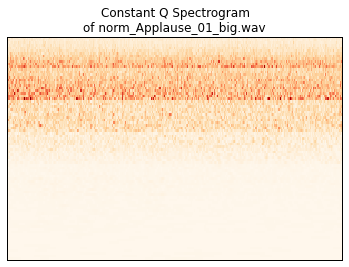
\includegraphics[width=\textwidth]{figures/cqt_applause.png}
      \caption{Constant Q spectrogram of an applause sound sample.}
      \label{fig:cqt-applause}
    \end{subfigure}
    \hfill 
    \begin{subfigure}[b]{0.3\textwidth}
      \centering
      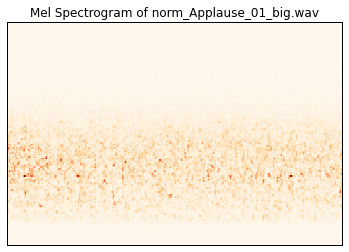
\includegraphics[width=\textwidth]{figures/mel_applause.png}
      \caption{Mel spectrogram of an applause sound sample.}
      \label{fig:cqt-applause}
    \end{subfigure}
        \hfill 
    \begin{subfigure}[b]{0.3\textwidth}
      \centering
      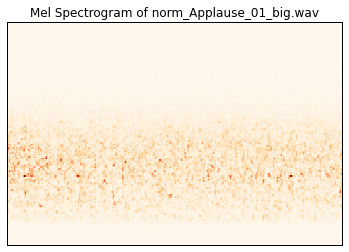
\includegraphics[width=\textwidth]{figures/mel_applause.png}
      \caption{Short Term Fourier Transform spectrogram of an applause sound sample.}
      \label{fig:cqt-applause}
    \end{subfigure}
    
    \caption{Three different spectrograms of the same sound sample of applause.}
    \label{fig:spectrogramCompare}
  \end{figure*}
  
    \begin{figure*}[hbt]
    \centering
    \begin{subfigure}[b]{0.45\textwidth}
      \centering
      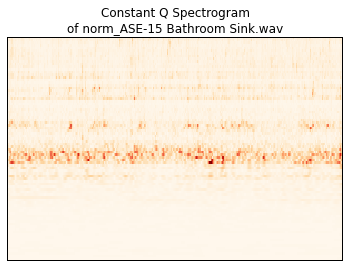
\includegraphics[width=\textwidth]{figures/cqt_bathroom_sink.png}
      \caption{Constant Q spectrogram of a bathroom sink.}
      \label{fig:cqt-applause}
    \end{subfigure}
    \hfill 
    \begin{subfigure}[b]{0.45\textwidth}
      \centering
      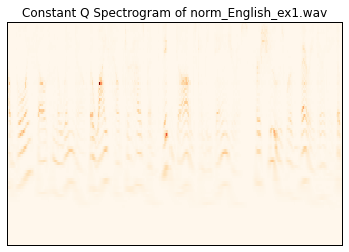
\includegraphics[width=\textwidth]{figures/cqt_english.png}
      \caption{Constant Q spectrogram of a person speaking English.}
      \label{fig:cqt-applause}
    \end{subfigure}
    \\
        \begin{subfigure}[b]{0.45\textwidth}
      \centering
      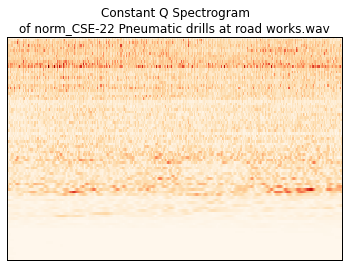
\includegraphics[width=\textwidth]{figures/cqt_pneumatic_drills.png}
      \caption{Constant Q spectrogram of pneumatic drills.}
      \label{fig:cqt-applause}
    \end{subfigure}
    \hfill 
    \begin{subfigure}[b]{0.45\textwidth}
      \centering
      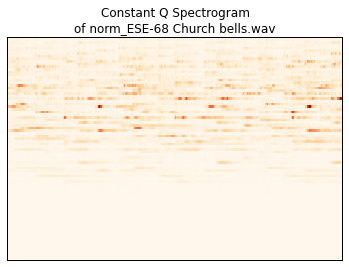
\includegraphics[width=\textwidth]{figures/cqtChurchBells.png}
      \caption{Constant Q spectrogram of church bells.}
      \label{fig:cqt-applause}
    \end{subfigure}
    \\
    \begin{subfigure}[b]{0.45\textwidth}
      \centering
      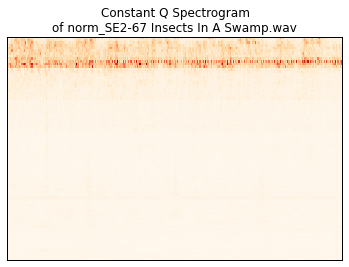
\includegraphics[width=\textwidth]{figures/cqt_insects.png}
      \caption{Constant Q spectrogram of insects in a swamp.}
      \label{fig:cqt-applause}
    \end{subfigure}
    \hfill 
    \begin{subfigure}[b]{0.45\textwidth}
      \centering
      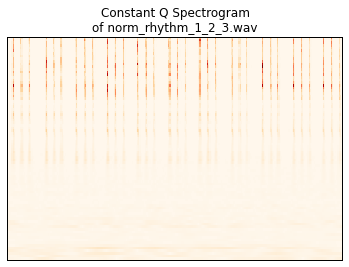
\includegraphics[width=\textwidth]{figures/cqt_rythm123.png}
      \caption{Constant Q spectrogram of a tapped rhythm.}
      \label{fig:cqt-applause}
    \end{subfigure}
    \caption{Constant Q spectragrams of a variety of different sounds. The left column contains sound textures and the right does not.}
    \label{fig:spectrograms}
  \end{figure*}

We performed a linear regression with $L_1$ regularization with all of our features. Half of the data was randomly selected to be used as training data, one quarter was reserved for a validation step to select our regularization constant, and a quarter was reserved to determine our final r-squared values. \xxx{talk about feature normalization}

\xxx{Describe how we set up our feature extraction. How we set up our learning. What our dataset is. Any other important process things.}

\section{Results}
\label{sec:results}

When we ran LASSO regressions, we consistently found that two features were of the most predictive value: the RMS energy of a sound and the time homogeneity of the RMS energy. A linear regression with either one of these features had $R^2$ of, on average, $.45$ on the test set. For sufficiently high regularization parameters, they were the only nonzero regression coefficients.

    \begin{figure*}[hbt]
    \centering
    \begin{subfigure}[b]{0.45\textwidth}
      \centering
      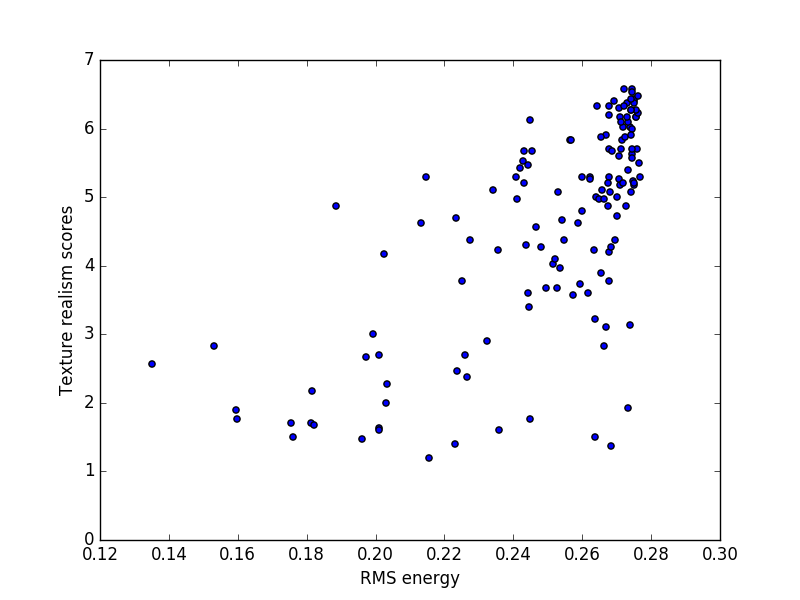
\includegraphics[width=\textwidth]{figures/rms_energy.png}
      \caption{Sound realism vs. RMS energy}
      \label{fig:rmsenergy}
    \end{subfigure}
    \hfill 
    \begin{subfigure}[b]{0.45\textwidth}
      \centering
      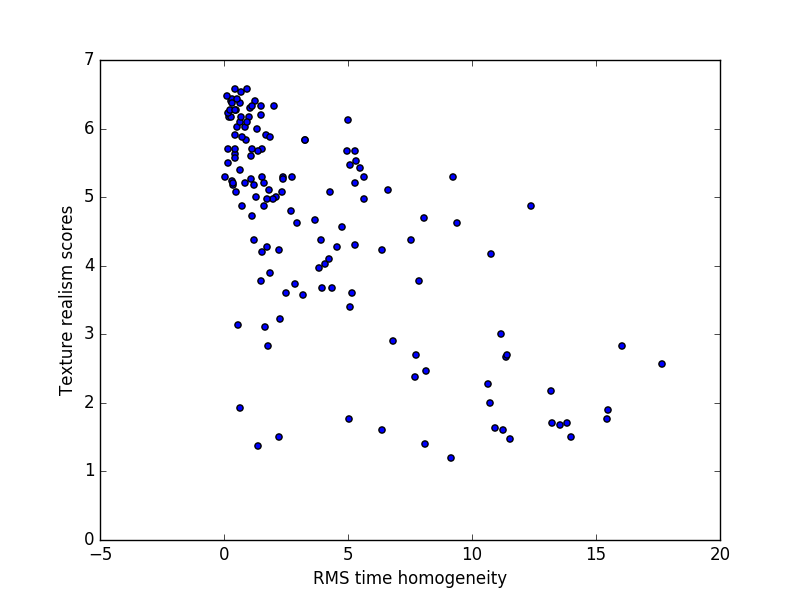
\includegraphics[width=\textwidth]{figures/rms_time_homogeneity.png}
      \caption{Sound texture realism vs. RMS time homogeneity}
      \label{fig:rmshomog}
    \end{subfigure}
    \\
        \begin{subfigure}[b]{0.45\textwidth}
      \centering
      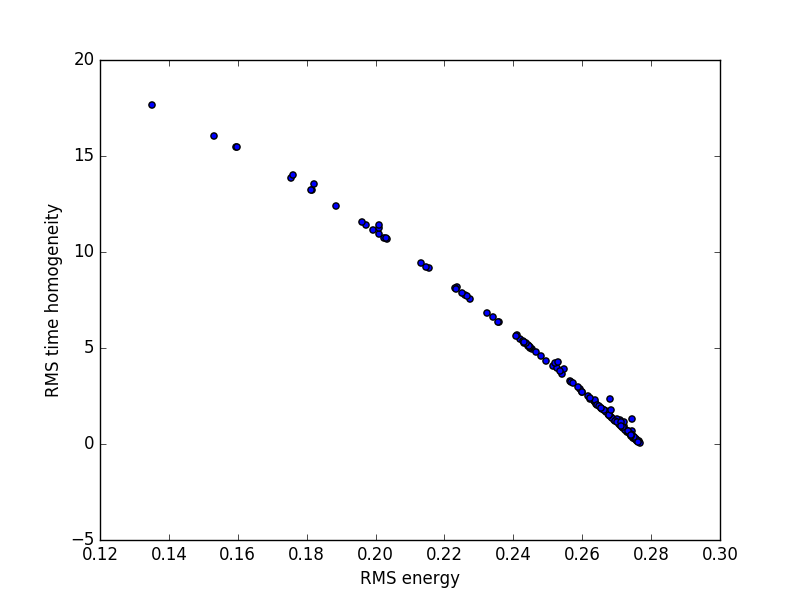
\includegraphics[width=\textwidth]{figures/rms_homogeneity_vs_energy.png}
      \caption{RMS time homogeneity vs. RMS energy}
      \label{fig:homogvsenergy}
    \end{subfigure}
    \end{figure*}

    While this early success seemed promising, we realized that it was, in fact, a problem. The RMS energy of a sound is essentially its loudness. As seen in Figure~\ref{fig:rmsenergy}, the louder the recording, the more like a sound texture it was.

    Because the degree to  which a sound is a sound texture is not based on how loud it is played, we assume that this is because of an artifact in how the sounds were recorded. Many things  that are clearly sound textures are quite loud (e.g.,  applause) or were likely recorded with a microphone close to the source of the sound (e.g., running water). On the other hand, sounds that are definitely not sound textures, like speech or church  bells, may have been recorded at more of a distance.

    In order to control for this effect, we normalized our recordings so that they had the same amplitude using the \texttt{librosa} Python package.

\xxx{What correlated and what didn't? What feature (ensemble) lead to a good classifier?}

\section{Conclusion}

Out of the large number of features investigated, we've shown that none of them have predictive power when we normalized the amplitudes of our sound samples to fall in the same range. Although we have only ruled out their usefulness in predicting sound textures, it seems unlikely that they will be generally useful in other types of audio classification. Further, this negative result has implications in the understanding of sound textures and human audition. It suggests that one informal conjecture about the nature of sound textures is incorrect. This will hopefully spur a refinement of ideas and definitions surrounding sound textures and provide a useful piece of evidence when considering how to move forward. One might now believe the decision to throw away temporal information about an audio signal to be more nuanced than previously thought and hopefully further work on features such as temporal coincidence, reverberation, natural harmonics, and temporal regularity will now be increasingly motivated.

There are a number of future directions left open by this paper. First, the space of reasonable features has not been fully explored and could still lead to useful features for classification or more insight into the nature of sound textures. These features include: other standard compression algorithms, the entropy of the audio signals, the Kolmogorov complexity of the audio signal, rank estimation of the audio signal, temporal homogeneity of the cross-band correlations, and different sparsity estimation criteria. Although these features are all related, they are certainly not the same and the authors know of no way to rule them out without direct investigation. Another possible direction is the integration of these features with existing audio classification methods to attempt to improve performance in more complex settings. We do not believe this is likely to be a fruitful search; however, the domain of attempting to classify the texturalality of sound is very narrow compared to the entirety of computer sound classification. Third, there is still much to be understood about the nature of these features and what they do tell us about an audio file. The authors would have been interested to look at the correlation between features and examples where these notions do and do not line up. Understanding when things like sparsity and compressibility differer might hold new insight into signal characteristics. Finally, there still remain important questions about the nature of human perception of sound textures. Now that we've ruled out a number of characterizing features, the question of what makes something a sound texture is even more tantalizing. 

\section*{Acknowledgments}

We thank Professor Josh McDermott for his support in answering our questions about his and Simoncelli's research and for providing us with their dataset. We also thank the course staff of 6.867 for their instruction and support this semester. In particular, we appreciate Marzyeh Ghassemi's advice and guidance in shaping our project plan.

\later{
\section{Dataset}
\label{sec:dataset}
Dataset with realism ratings from \cite{McDermott2011926}.

 Insects in swamp
6.57 

 Heavy rain on hard surface
6.53 

 Frogs
6.53 

 Rain
6.47 

 Applause 

 big room
6.43 

 Radio static
6.43 

 Stream
6.43 

 Jungle rain
6.40 

 Air conditioner
6.40 

 Stream near small waterfall
6.37 

 Frogs
6.37 

 Frogs and insects
6.37 

 Frying eggs
6.33 

 Frogs
6.33 

 Wind 

 blowing
6.33 

 Wind 

 whistling
6.33 

 Insects during day in South
6.30 

 Radio static
6.30 

 Frogs
6.30 

 Heavy rain falling and dripping
6.27 

 Applause 

 large crowd
6.27 

 River running over shallows
6.27 

 Construction site ambience
6.23 

 Waterfall
6.20 

 Sparrows 

 large excited group
6.17 

 Pneumatic drills
6.17 

 Small river
6.17 

 Fast running river
6.17 

 Rain in woods
6.13 

 Water trickling into pool
6.10 

 Bathroom sink
6.10 

 Water running into sink
6.03 

 Frying bacon
6.03 

 Rain in ihe woods
6.00 

 Fire 

 forest inferno
5.97 

 Birds in forest
5.90 

 Linotype
5.90 

 Bee swarm
5.90 

 Applause
5.90 

 Bath being drawn
5.90 

 Rustling paper
5.87 

 Train speeding down railroad tracks 

 steam
5.87 

 Rattlesnake rattle
5.83 

 Fire 

 burning room
5.83 

 Bubbling water
5.83 

 Fire 

 burning room
5.83 

 Thunder and rain
5.73 

 Fire
5.70 

 Wind 

 moaning
5.70 

 Bulldozer
5.70 

 Babble
5.70 

 Fire
5.70 

 Wind 

 spooky
5.70 

 Water lapping gently
5.67 

 Shaking coins
5.67 

 Helicopter
5.67 

 Seagulls
5.63 

 Crunching cellophane
5.63 

 Sander
5.60 

 Radio static
5.60 

 Teletype 

 city room
5.57 

 Steam shovel
5.53 

 Pigeons cooing
5.50 

 Metal lathe
5.47 

 Bee swarm
5.47 

 Lapping waves
5.43 

 Geese cackling
5.40 

 Train speeding down railroad tracks 

 Diesel
5.30 

 Lake shore
5.30 

 Sanding by hand
5.30 

 Blender
5.30 

 Teletype
5.30 

 Birds in tropical forest
5.27 

 Drumroll
5.27 

 Surf hitting beach
5.23 

 Industrial machinery
5.20 

 Crowd noise
5.20 

 Rolling coin
5.20 

 Ducks quacking
5.20 

 WWII bomber plane
5.17 

 Applause
5.17 

 Idling boat
5.17 

 Jackhammer
5.10 

 Brushing teeth
5.10 

 Horse trotting on cobblestones
5.07 

 Scratching beard
5.07 

 Printing press
5.07 

 Writing with pen on paper
5.00 

 Train locomotive 

 steam engine
5.00 

 Helicopter fly by
4.97 

 Pouring coins
4.97 

 Motorcycle idling
4.97 

 Fire
4.93 

 Crumpling paper
4.87 

 Ship anchor being raised
4.87 

 Jingling keys
4.87 

 Electric adding machine
4.80 

 Horse walking in snow
4.73 

 Cymbals shaking
4.70 

 Fire 

 in chimney
4.67 

 Tambourine shaking
4.67 

 Pouring coins
4.63 

 Rhythmic applause
4.63 

 Cat lapping milk
4.57 

 Seaside waves
4.43 

 Rustling paper
4.37 

 Horse pulling wagon
4.37 

 Vacuum cleaner
4.37 

 Horse and carriage
4.30 

 Power saw
4.30 

 Tire rolling on gravel
4.27 

 Horse and buggy
4.27 

 Steam engine
4.23 

 Cement mixer
4.23 

 Power saw
4.23 

 Castanets
4.23 

 Ox cart
4.20 

 Battle explosions
4.17 

 Chickens squawking
4.10 

 Rubbing cloth
4.03 

 Rain beating against window panes
3.97 

 Typewriter 

 IBM electric
3.90 

 Lawn mower
3.77 

 Gargling
3.77 

 Horse gallop on soft ground
3.73 

 Applause 

 foreground clapper
3.67 

 Sawing by hand
3.67 

 Crumpling paper
3.60 

 Wolves howling
3.60 

 Fast breathing
3.57 

 Dogs
3.40 

 Out of breath
3.23 

 Windshield wipers
3.20 

 Pile driver
3.13 

 Silly mouth noise
3.10 

 Large diner
3.00 

 Filing metal
2.90 

 Typewriter 

 manual
2.83 

 Fire alarm bell
2.83 

 Knife sharpening
2.83 

 Typewriter 

 old
2.70 

 Pile driver
2.70 

 Clock ticking
2.67 

 Jogging on gravel
2.67 

 Castanets
2.57 

 Hammering copper
2.47 

 Laughter
2.47 

 Tapping rhythm
2.37 

 Running up stairs
2.27 

 Typewriter 

 IBM selectric
2.17 

 Men marching together
2.00 

 Tapping on hard surface
1.93 

 Railroad crossing
1.90 

 Tapping 1

2
1.77 

 Wind chimes
1.77 

 Corkscrew against desk edge
1.70 

 Reverse drum beats 

 snare
1.70 

 Tapping  1

2

3
1.67 

 Snare drum beats
1.63 

 Walking on gravel
1.60 

 Snare rimshot sequence
1.60 

 Music 

 Apache drum break
1.50 

 Music 

 mambo
1.50 

 Bongo loop
1.47 

 Firecrackers
1.40 

 Person speaking French
1.37 

 Church bells
1.20 

 Person speaking Engli
}





% bibliography
\bibliographystyle{abbrv}
\bibliography{SoundTexturesBib}
\end{document}

